\documentclass[aspectratio=169]{beamer}
\setbeamertemplate{navigation symbols}{}
\usepackage{color,amsmath,comment, subfigure}
\usepackage{booktabs}
\usepackage{url}

\def\imagetop#1{\vtop{\null\hbox{#1}}} %http://tex.stackexchange.com/questions/23521/tabular-vertical-alignment-to-top

%%%%%%%%%%%%%%%%%%%%%%%%%%
\title[]{Lecture 23: Who knows what about who?}
\author[]{Matthew J. Salganik}
\institute[]{Sociology 204: Social Networks\\Princeton University}
\date[]{
2/2 Secrets
\vfill

\begin{flushleft}
\vspace{0.6in}

\includegraphics[width=0.1\textwidth]{figures/cc.png}
\end{flushleft}
}

\note{
More compare and contrast of three studies:
- design (interview of alters vs guess what alter will say, game of contacts doesn't ask actual alter info)
- goals (basic vs applied)
}

\begin{document}
%%%%%%%%%%%%%%%%%%%%%%%%%%%
\frame{\titlepage}
%%%%%%%%%%%%%%%%%%%%%%%%%%%
\begin{frame}

\begin{itemize}
\item your perception of the social world is distorted
\pause
\item your perception of your own social world is distorted
\end{itemize}

\pause 
Why do we care?

\begin{itemize}
\item important for scale-up method \pause
\item interesting \pause
\item impacts social influence \pause
\item potentially creates social stasis 
\end{itemize}

\end{frame}
%%%%%%%%%%%%%%%%%%%%%%
\begin{frame}

\LARGE{Cowan: secrets and self-fulfilling illusions}

\end{frame}
%%%%%%%%%%%%
\begin{frame}

Contact hypothesis: when individuals come into contact with a stigmatized outgroup, prejudice decreases 

\vfill

What if secrets prevent us from realized that we are already in connect with stigmatized outgroups?

\end{frame}
%%%%%%%%%%%%
\begin{frame}

Survey of random sample of Americans to measuring hearing and telling about two outcomes
\begin{itemize}
\item having an abortion
\item having a miscarriage
\end{itemize}

\end{frame}
%%%%%%%%%%%%
\begin{frame}

Hypothesis 1: Among concealable characteristics, the less stigmatized the characteristic the more people will hear about it \pause

\begin{itemize}
\item 75\% of Americans report knowing someone who has had a miscarriage
\item 50\% of Americans report knowing someone who had an abortion 
\end{itemize}
\pause
\begin{itemize}
\item Estimated that nearly 20\% of recognized pregnancies end in abortion
\item Estimated that 13\% of recognized pregnancies end in miscarriage
\end{itemize}

\end{frame}
%%%%%%%%%%%%%
\begin{frame}

\begin{center}
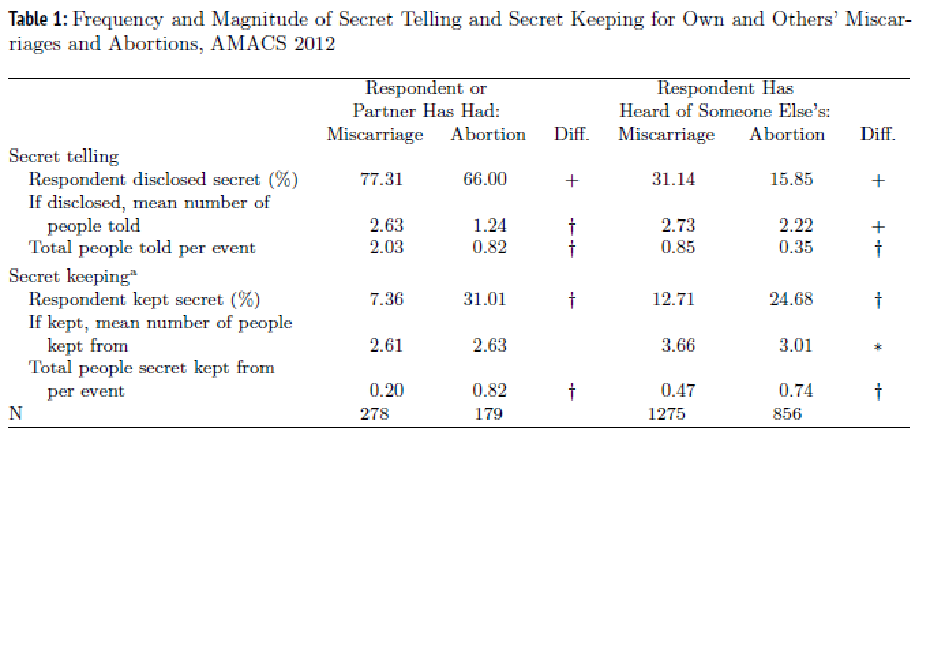
\includegraphics[width=1\textwidth]{figures/cowan_secrets_2014_tab1}
\end{center}

\vfill
\begin{itemize}
\item Difference in hearing is because miscarriage secrets are told to more people and concealed from fewer people
\end{itemize}
\end{frame}
%%%%%%%%%%%%
\begin{frame}

Hypothesis 2: Among concealable characteristics, people who hold positive attitudes toward the characteristics are more likely to hear about it

\pause

\begin{center}
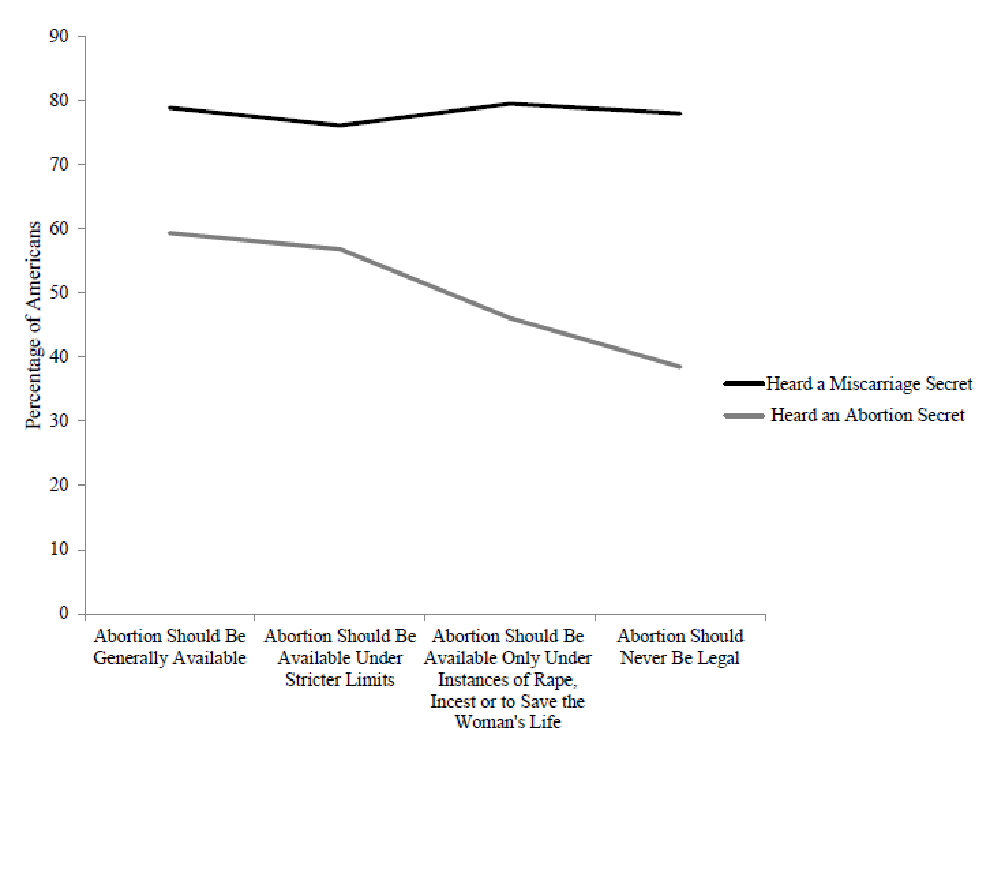
\includegraphics[width=0.6\textwidth]{figures/cowan_secrets_2014_fig1}
\end{center}

\begin{itemize}
\item Comparison between abortion and miscarriage is key here
\item Cowen thinks attitude change is unlikely to explain this pattern
\end{itemize}

\note{
attitude change is unlikely to explain this pattern she says
}

\end{frame}
%%%%%%%%%%%%
\begin{frame}

Hypothesis 3: Among concealable characteristics, the more stigmatized the more likely to be disclosed to those who are accepting

\vfill
\pause

Supported by:
\begin{itemize}
\item open-ended responses to survey
\item intake data from abortion clinic
\end{itemize}

\end{frame}
%%%%%%%%%%%%%%%%%
\begin{frame}

What if secrets prevent us from realized that we are already in connect with stigmatized outgroups?\\ \pause

Information ends up where it will have the least effect leading to social stasis

\end{frame}
%%%%%%%%%%%%
\begin{frame}

\LARGE{Goel et al: Real and perceived attitude homophily}

\vfill
Not assigned

\end{frame}
%%%%%%%%%%%%%%%%%%%%%%%%%
\begin{frame}

homophily: ``love of the same'' (offline filter bubble)\\

People tend to be connected to people who are similar to them:
\begin{itemize}
\item sociodemographic homophily
\item attitude homophily
\end{itemize}

\vfill

Maybe our attitudes are not as similar as we think to our friends?

\end{frame}
%%%%%%%%%%%%%%%%%%%%%%%
\begin{frame}

``Would you go to a One Direction concert if you were given free tickets?'' \\

Alice and Bob are friends:
\begin{itemize}
\item Alice answers question about Alice
\item Alice answers question about Bob
\item Bob answers question about Bob
\item Bob answers question about Alice
\end{itemize}

From patterns, we can estimate actual agreement and perceived agreement

\end{frame}
%%%%%%%%%%%%%%%%%%%%%%%
\begin{frame}

Facebook app used ``social graph''; kind of like a social quiz

\begin{center}
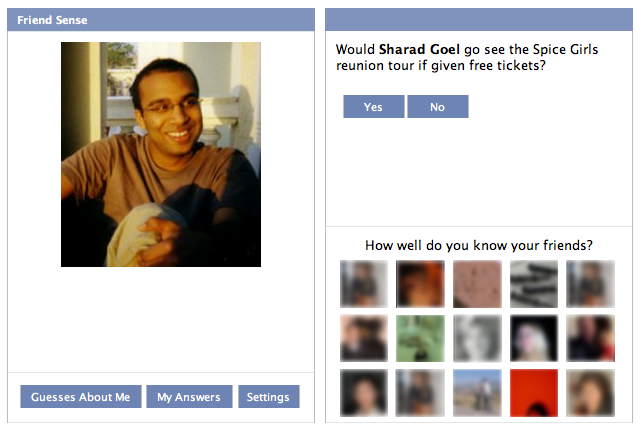
\includegraphics[width=0.7\textwidth]{figures/friendsense.png}
\end{center}

\end{frame}
%%%%%%%%%%%%%%%%%%%%%%
\begin{frame}

\begin{center}
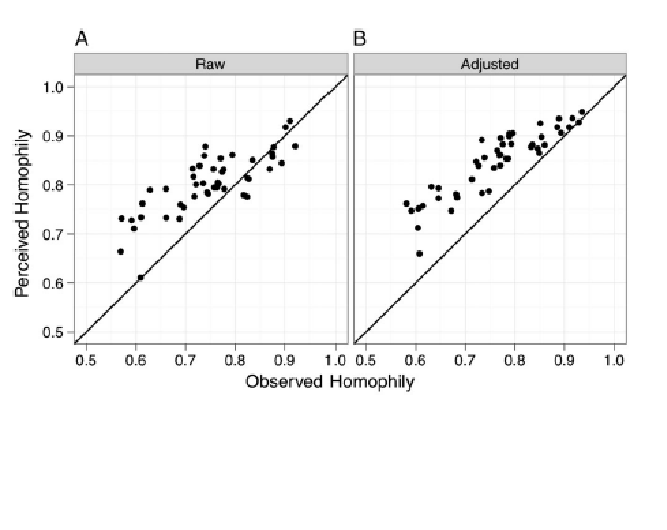
\includegraphics[width=0.7\textwidth]{figures/goel_real_2010_fig4}
\end{center}

\begin{itemize}
\item For almost all questions considered, perceived agreement is higher than observed agreement (although it depends a bit on statistical adjustments)
\end{itemize}

\end{frame}
%%%%%%%%%%%%%%%%%%%%%%%%
\begin{frame}

\begin{center}
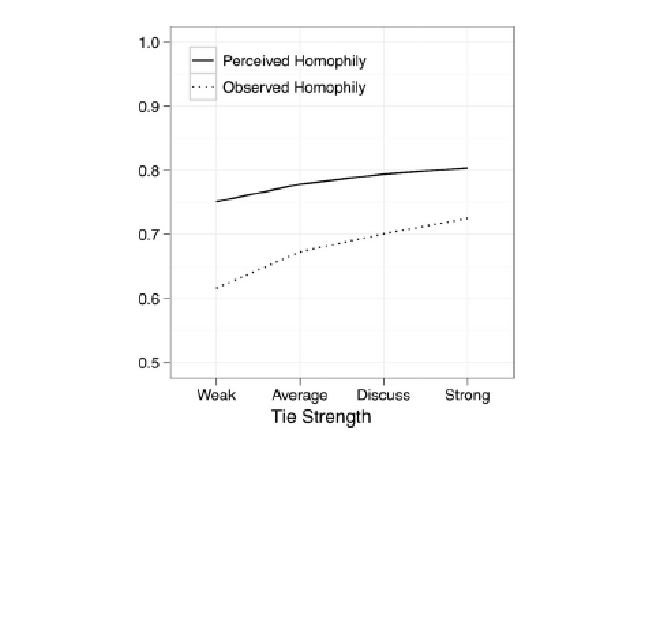
\includegraphics[width=0.5\textwidth]{figures/goel_real_2010_fig3}
\end{center}

\begin{itemize}
\item Perceived agreement is higher than observed agreement for all different tie strengths
\end{itemize}

\end{frame}
%%%%%%%%%%%%%%%%%
\begin{frame}

\begin{center}
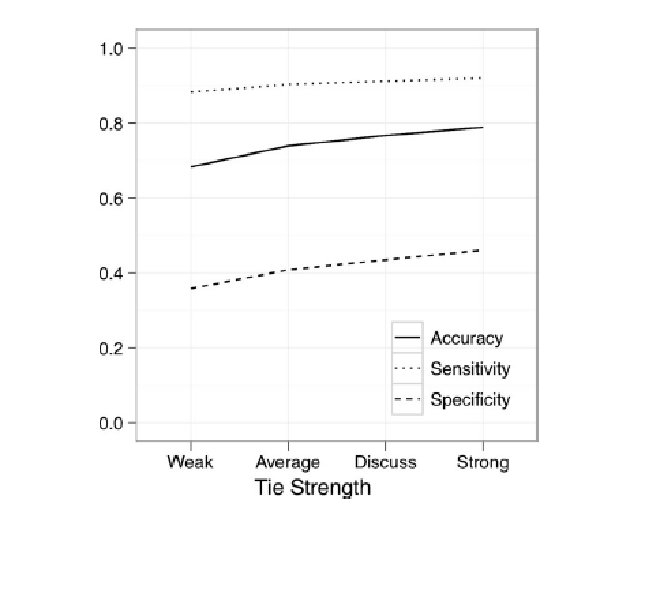
\includegraphics[width=0.3\textwidth]{figures/goel_real_2010_fig6}
\end{center}

People are bad at detecting disagreement
\begin{itemize}
\item Accuracy = p(correct guess)
\item Sensitivity = p(correct guess given agreement)
\item Specificity = p(correct guess given disagreement)
\end{itemize}

\end{frame}
%%%%%%%%%%%%%%%%%
\begin{frame}

\begin{tabular}{ccc}
\imagetop{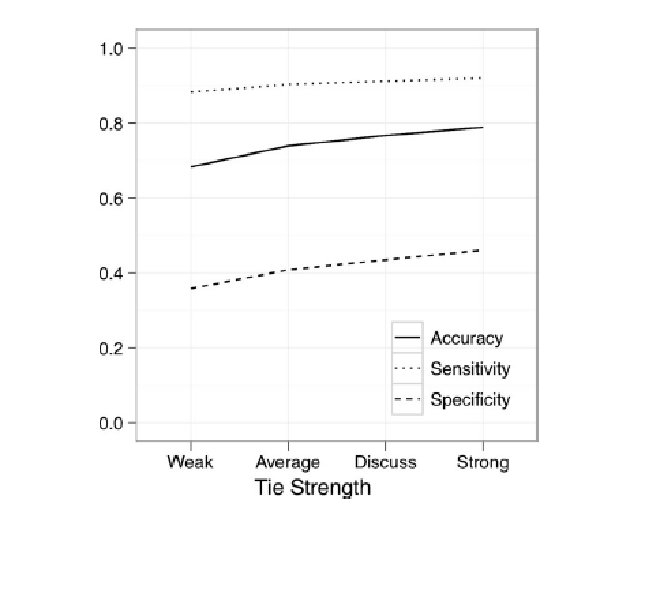
\includegraphics[width=0.3\textwidth]{figures/goel_real_2010_fig6}} &
\pause
\imagetop{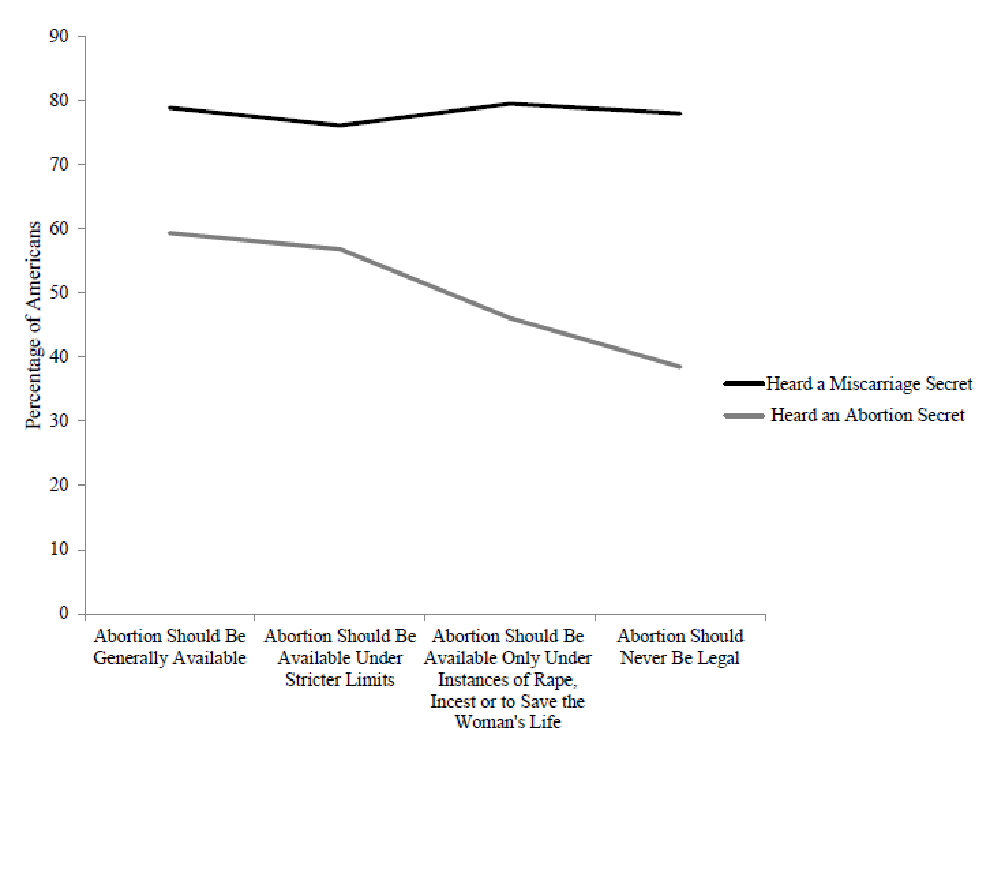
\includegraphics[width=0.3\textwidth]{figures/cowan_secrets_2014_fig1}} &
\pause
\imagetop{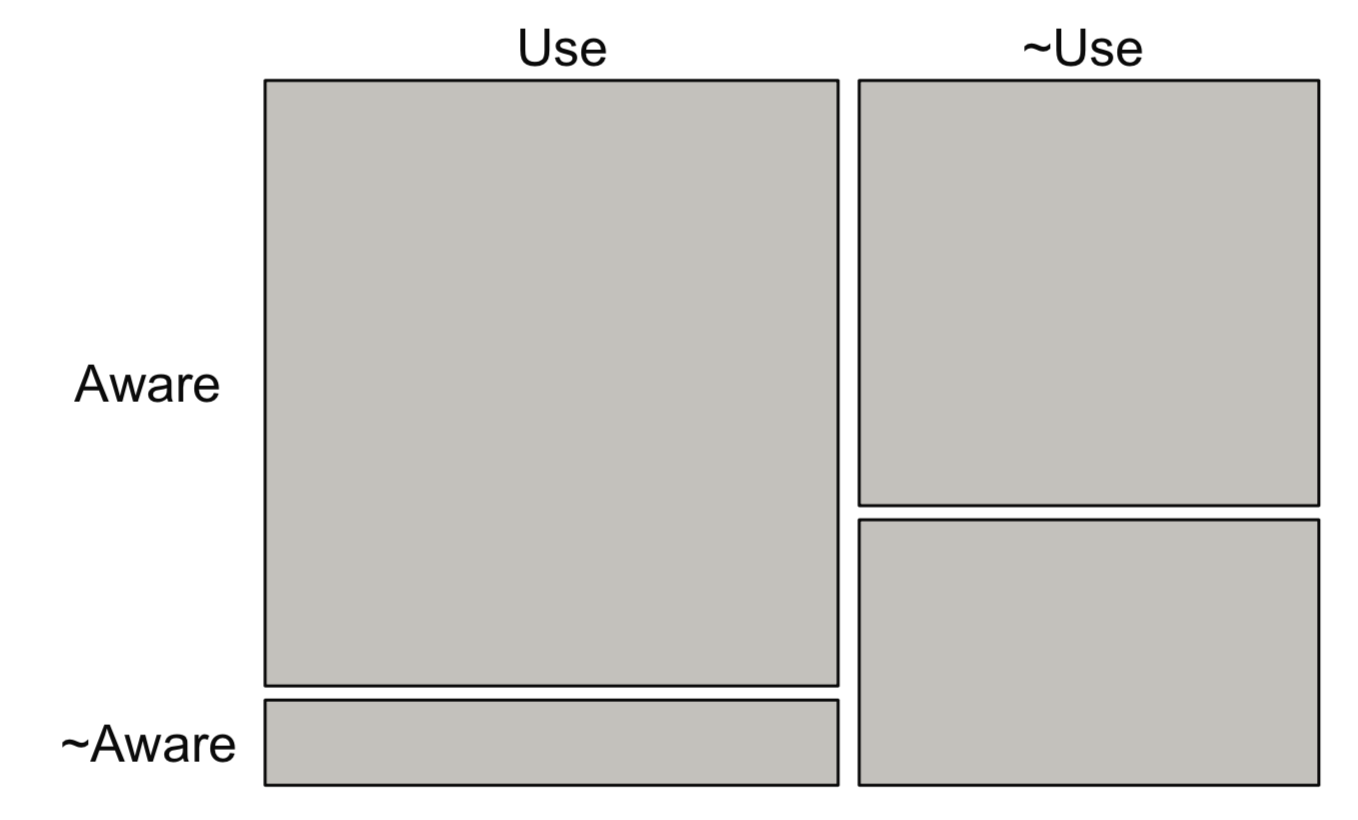
\includegraphics[width=0.3\textwidth]{figures/salganik_game_2011_fig3}}\\
\end{tabular}

\end{frame}
%%%%%%%%%%%%%%%%%%
\begin{frame}

\begin{center}
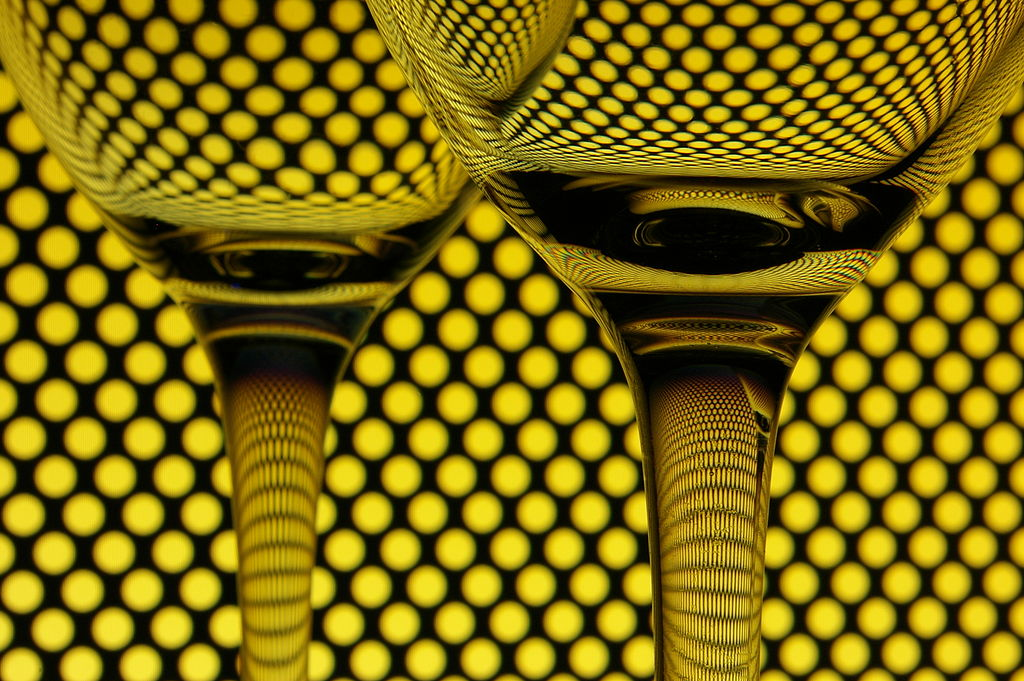
\includegraphics[width=0.8\textwidth]{figures/distortion.jpg}
\end{center}

\vfill
\tiny{\url{https://commons.wikimedia.org/wiki/File:Uniformity.jpg}}

\end{frame}
%%%%%%%%%%%%%%%%%%%
\begin{frame}

Stepping back:
\begin{itemize}
\item your beliefs about the attitude of your friends are probably systematically distorted \pause
\item systematic biases in information awareness may promote stability of attitudes \pause
\item systematic biases can mess up scale-up estimates, but these can be measured
\end{itemize}

\end{frame}
%%%%%%%%%%%%%%%%%%%


\end{document}
